\section{Construction and Preprocessing Results}

The following results concern actual dataset inventories and retained corpus/tokenizer measurements. They
are not simulated model responses. Counts summarize the constructed collection; they are not random-sample
estimates of a population accuracy, so model-performance confidence intervals and significance tests are
inapplicable. The 33 split-by-size dataset records and the 236 native lexical publication records supply
every numerical display in this section.

\subsection{Dataset scale and the distinction between units}

The collection contains 3,000 latent orders, 23,200 source queries, 5,637,600 prompt identities, and
7,819,200 comparison cells (Table~\ref{tab:inventory}). Source-order allocation is 450 training, 450
development, 300 pilot, and 1,800 test orders. The training allocation spans the frozen size grid, while optional training selects only
$n \le 128$; split membership does not imply selection for optimization. These counts describe different
units: each source order supports multiple queries, and each query expands into 243
language/name/relation/presentation identities. Comparison cells additionally include matched contrasts and
endpoint-to-interior comparisons. They are not 7.8 million independent reasoning trials.

\begin{table}[t]
  \centering
  \caption{Verified dataset inventory. Orders are source chains; queries and presentations are dependent
  derivatives. Presentation counts describe the frozen design, not completed model calls.}
  \label{tab:inventory}
  \small
  \begin{tabular}{@{}lrrrr@{}}
    \toprule
    Split & Orders & Queries & Presentations & Pairing cells \\
    \midrule
    Training    &   450 &  3\,550 &   862\,650 & 1\,197\,450 \\
    Development &   450 &  3\,550 &   862\,650 & 1\,197\,450 \\
    Pilot       &   300 &  1\,900 &   461\,700 &   634\,500 \\
    Frozen test & 1\,800 & 14\,200 & 3\,450\,600 & 4\,789\,800 \\
    \midrule
    Total       & 3\,000 & 23\,200 & 5\,637\,600 & 7\,819\,200 \\
    \bottomrule
  \end{tabular}
\end{table}

\begin{figure}[t]
  \centering
  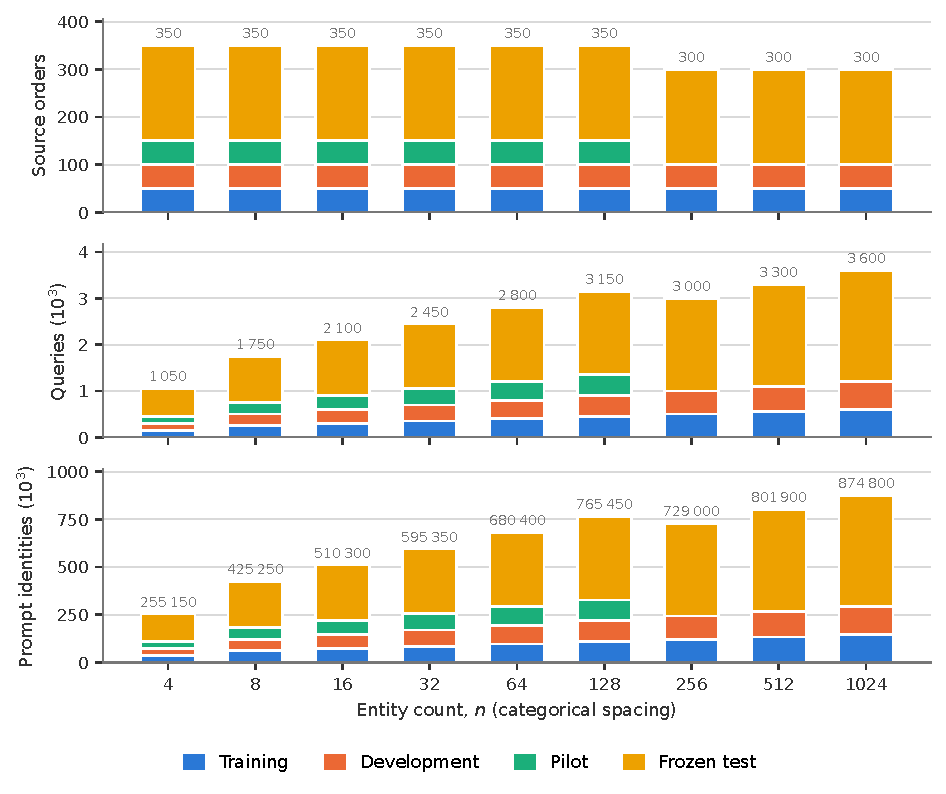
\includegraphics[width=\linewidth]{figures/manuscript/fig2_construction_counts.pdf}
  \caption{Verified construction counts by size and split. Source orders and derived queries/prompts are
  different units. This figure contains no model predictions.}
  \label{fig:construction}
\end{figure}

Figure~\ref{fig:construction} shows why entity count, independent sample size, and workload must be kept
separate. The full-test number of source orders is fixed per $n$, while the number of feasible distance
conditions grows with $n$. Pilot coverage stops at $n = 128$. The larger prompt workload at high $n$
therefore reflects both presentation length and the design's query expansion; it is not evidence that a
model performed more logical steps.

\subsection{Independent corpus frequency and morphological realization}

The retained lexical measurement uses the three corpus partitions of UD Turkish BOUN release r2.18, revision
\texttt{0def94a229dcbc28d32192b0138b560c075c6d87}, under CC-BY-SA-4.0. BOUN's resource design and annotation
context are described by \citet{turk2022boun}; the locked release, not the paper's headline counts alone,
defines our measurements. Retained coverage includes 9,761 sentences, 101,052 eligible surface tokens, and
104,424 eligible lemma positions. The recorded normalization uses Unicode NFC and Turkish-aware case folding
(I~$\to$~ı, İ~$\to$~i), with exact normalized $n$-gram matching. Surface $n$-gram opportunity counts differ
with expression length; rates must retain their own denominators.

All 18 canonical inflected relation expressions have measured surface count zero, while their recorded lemma
counts range from 10 to 390. Table~\ref{tab:lemma} lists the paired forward/inverse lemma counts, and
Figure~\ref{fig:lemma} reports those values and directions. A measured zero is
a property of this corpus and matching rule; it is not missing data and does not show that the expression is
ungrammatical or absent from all Turkish. Conversely, a positive count of a lemma such as \emph{üst} can
include senses outside the intended ordering relation. Surface and lemma frequencies answer different
questions.

For every zero surface count, an unsmoothed $\log_{10}$ frequency is undefined. Forward/inverse ratios with
zero inverse denominators are likewise undefined; $0/0$ is not set to one. Smoothing could define a
different exploratory feature but would require an explicit new measurement specification. We retain the
original zero/undefined distinction. These findings motivate careful lexical feature construction rather
than a claim that lower frequency causes a reasoning error.

\begin{figure}[t]
  \centering
  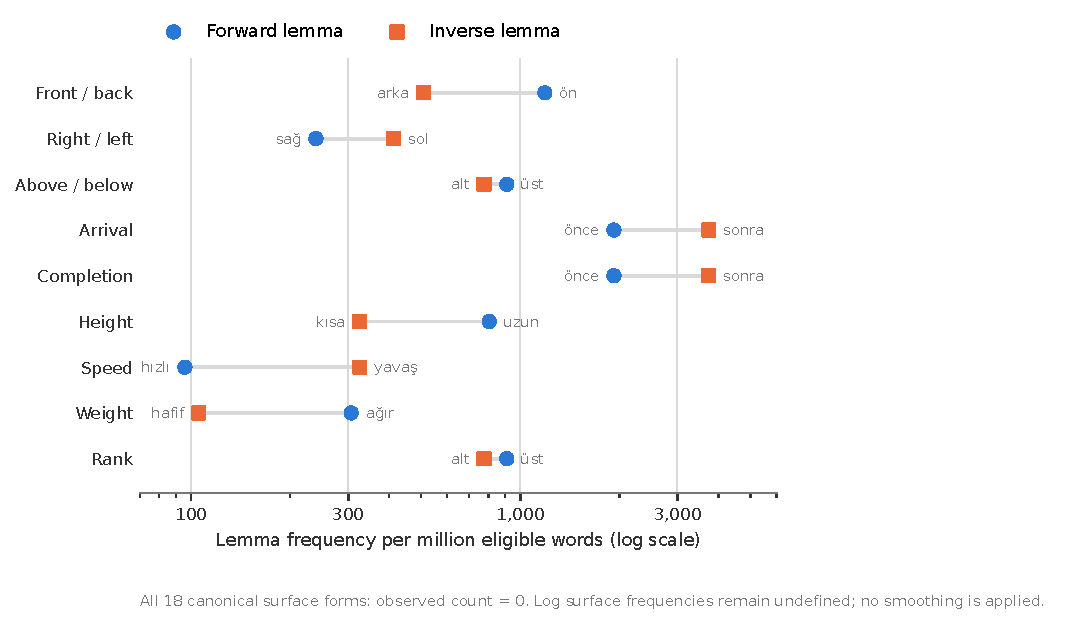
\includegraphics[width=\linewidth]{figures/manuscript/fig3_lemma_frequencies.pdf}
  \caption{Observed canonical surface counts and lemma frequency proxies for the nine forward/inverse
  relation pairs. Surface zeros are measured zeros; lemma counts are not sense-disambiguated counts of the
  full relation expression. Lines connect paired forward and inverse proxies; they are not confidence
  intervals. No model outcome is represented.}
  \label{fig:lemma}
\end{figure}

\begin{table}[t]
  \centering
  \caption{Independent relation-lemma counts in UD Turkish BOUN r2.18 (104,424 eligible lemma tokens).
  These are lemma counts, not sense-disambiguated relation frequencies. All 18 canonical surface-form counts
  are zero. Shared lemmas recur across templates.}
  \label{tab:lemma}
  \small
  \begin{tabular}{@{}llrlrr@{}}
    \toprule
    Relation & Forward lemma & Count & Inverse lemma & Count & $f_F/f_I$ \\
    \midrule
    Front / back  & ön    & 124 & arka  &  53 & 2.34 \\
    Right / left  & sağ   &  25 & sol   &  43 & 0.58 \\
    Above / below & üst   &  95 & alt   &  81 & 1.17 \\
    Arrival       & önce  & 201 & sonra & 390 & 0.52 \\
    Completion    & önce  & 201 & sonra & 390 & 0.52 \\
    Height        & uzun  &  84 & kısa  &  34 & 2.47 \\
    Speed         & hızlı &  10 & yavaş &  34 & 0.29 \\
    Weight        & ağır  &  32 & hafif &  11 & 2.91 \\
    Rank          & üst   &  95 & alt   &  81 & 1.17 \\
    \bottomrule
  \end{tabular}
\end{table}

\subsection{Tokenizer measurements}

The isolated-vocabulary export has 216 records: six registered configurations, nine relations, two
directions, and two languages. Counts cover the GPT-4o encoding configuration, the three Qwen
configurations, and the two Llama configurations. The Llama tokenizer assets are license-gated upstream;
they were vendored at the registered immutable revisions after license acceptance, with every file verified
against its upstream Git object hash, rather than being inferred from another tokenizer (an earlier retained
measurement records them as explicitly unavailable). A tokenizer measurement does not mean that model
weights were loaded or that its answers were evaluated.

All 216 isolated-vocabulary records are measured (Table~\ref{tab:tokenizers}). Across the 18 matched
relation-term pairs in each configuration, the median Turkish/English term-token ratio is 2.75 for
the GPT-4o encoding, 2.25 for each Qwen configuration, and 2.00 for each Llama configuration; observed
ratios across configurations range from 0.75 to 6. These are medians of matched ratios, not ratios of
median token counts. They summarize the selected lexical inventory without inferential confidence
intervals.

\begin{table}[t]
  \centering
  \caption{Tokenizer preprocessing coverage, not inference results. Each configuration has 18 Turkish and 18
  English relation terms; ratios use matched isolated terms. The three Qwen configurations yield identical
  term counts, as do the two Llama configurations; neither family contributes independent tokenization
  samples.}
  \label{tab:tokenizers}
  \small
  \begin{tabular}{@{}lrrrr@{}}
    \toprule
    Configuration & Measured & Median TR & Median EN & Median TR/EN \\
    \midrule
    GPT-4o / o200k\_base  & 36/36 & 4.0 & 2.0 & 2.75 \\
    Qwen2.5-0.5B / HF     & 36/36 & 5.0 & 2.5 & 2.25 \\
    Qwen2.5-1.5B / HF     & 36/36 & 5.0 & 2.5 & 2.25 \\
    Qwen2.5-1.5B / vLLM   & 36/36 & 5.0 & 2.5 & 2.25 \\
    Llama3.2-1B / HF      & 36/36 & 4.0 & 2.5 & 2.00 \\
    Llama3.2-3B / HF      & 36/36 & 4.0 & 2.5 & 2.00 \\
    \bottomrule
  \end{tabular}
\end{table}

\begin{figure}[t]
  \centering
  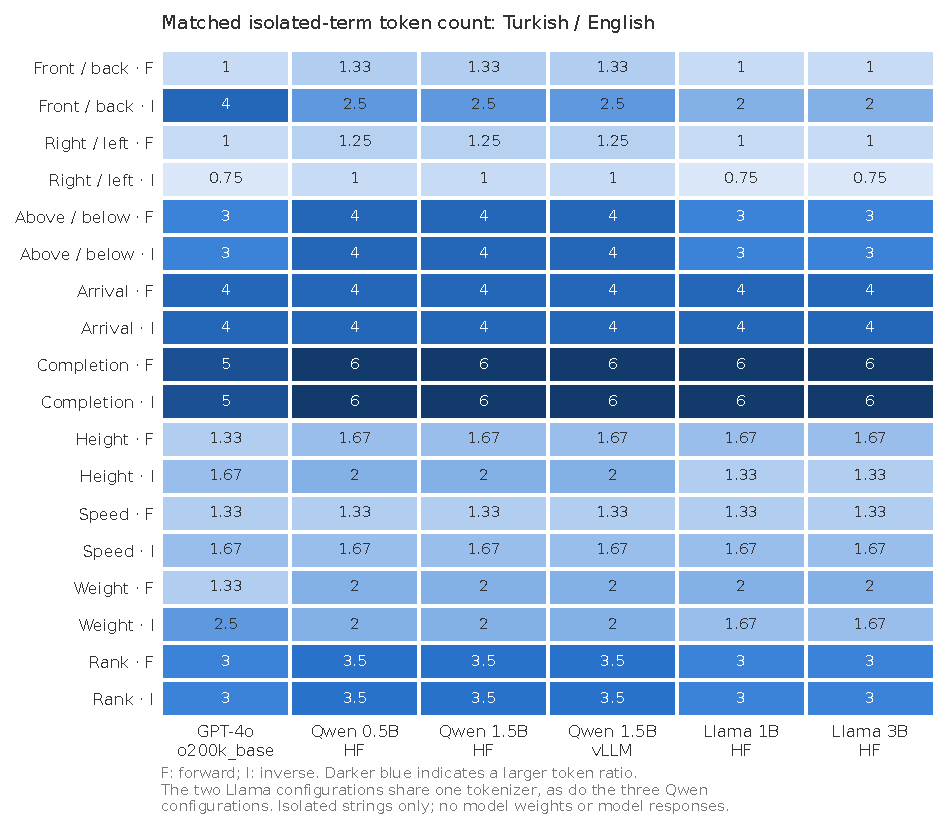
\includegraphics[width=0.94\linewidth]{figures/manuscript/fig4_token_ratios.pdf}
  \caption{Verified isolated relation-term tokenization. Matched Turkish/English measurements and
  forward/inverse differences describe the lexical strings and retained tokenizer assets; these are not
  model-performance comparisons.}
  \label{fig:tokens}
\end{figure}

Figure~\ref{fig:tokens} compares measured term tokenization across languages and directions on matched
lexical entries. Shared-tokenizer configurations are shown as configurations, not treated as independent
model families or independent replications. A ratio above one indicates a longer Turkish tokenization for
that lexical measurement and tokenizer. It does not imply a corresponding accuracy loss. Isolated
expressions, complete plain-text prompts, chat templates, and provider-billed usage have different scopes
\citep{rust2021tokenizer, ahia2023languages, petrov2023tokenizers}.

The corpus and tokenization audit provides features for RQ4; the executed pilot join
(Section~\ref{sec:pilot}) yields direction-specific diagnostics but cannot identify the
performance-association component from one relation family. The tokenized prompt preview is bounded to
$n = 4$; the isolated-term export should not be described as an analysis of full chat length across the
entire benchmark. Outcome analyses join by the exact latent/presentation coordinate and model/tokenizer
revision.

\subsection{What remains empirically unanswered}

Table~\ref{tab:availability} prevents preprocessing observations from being mistaken for answers to
RQ1--RQ5. The exploratory pilot evaluation of Section~\ref{sec:pilot} supplies the first genuine
accuracy-versus-$n$ curves, $R/D/U$ decompositions, and declared-family tests on the pilot split and one
relation family; the supplemental sweep of Section~\ref{sec:p1-local} extends them to all nine relation
families and four model scales; and the completed human review of Section~\ref{sec:review} backs the
sampled stimuli's grammaticality and meaning preservation. Confirmatory status still requires the
frozen-test design. The figures in the preceding subsections visualize actual construction/feature
measurements and a conceptual pipeline. No source-paper model scores are relabeled as Turkish-CBE results.

\begin{table}[t]
  \centering
  \caption{Outcome availability. NA is unavailable, not zero performance. ``Pilot (exploratory)'' denotes
  the executed pilot-split runs of Section~\ref{sec:pilot}; no confirmatory frozen-test estimate is
  reported.}
  \label{tab:availability}
  \small
  \begin{tabular}{@{}lp{0.47\linewidth}l@{}}
    \toprule
    Target & Required evidence & Current status \\
    \midrule
    Turkish--English gap        & Matched genuine answers and all-planned accuracy        & Pilot + sweep (exploratory) \\
    Morphosyntactic robustness  & Canonical/equivalent answers, $R/D/U$, coverage          & Pilot + sweep (exploratory) \\
    Complexity/distance profiles & Answers separated by $n$, $d$, and query type           & Pilot + sweep (exploratory) \\
    Lexical bias associations   & Direction-specific predictions joined to measured features & Pilot (diagnostics only) \\
    Stimulus linguistic validity & Two-reviewer sampled review with predeclared policy      & Completed (sampled) \\
    Reasoning/adaptation gains  & Matched intervention runs and recorded budgets           & Trained; evaluation gated \\
    \bottomrule
  \end{tabular}
\end{table}
